\hypertarget{construir-el-tutorial-de-gtk4}{%
\section{Construir el Tutorial de
Gtk4}\label{construir-el-tutorial-de-gtk4}}

\hypertarget{guuxeda-ruxe1pida}{%
\subsection{Guía rápida}\label{guuxeda-ruxe1pida}}

\begin{enumerate}
\def\labelenumi{\arabic{enumi}.}
\tightlist
\item
  Necesitas el sistema operativo linux, ruby, make, pandoc y latex
  instalados.
\item
  Descarga este repositorio y descomprime el archivo.
\item
  Cambia al directorio superior de los archivos fuente.
\item
  Escribe \texttt{rake\ html} para crear archivos html. Los archivos se
  crearán dentro de la carpeta \texttt{docs}.
\item
  Escribe \texttt{rake\ pdf}para crear el pdf. El archivo se creará
  dentro de la carpeta \texttt{latex}.
\end{enumerate}

\hypertarget{prerequisitos}{%
\subsection{Prerequisitos}\label{prerequisitos}}

\begin{itemize}
\tightlist
\item
  Sistema operativo Linux Los programas de este repositorio han sido
  probados en Ubuntu 21.04
\item
  Descarga los archivos en el repositorio. Hay 2 maneras de hacer la
  descarga.
\end{itemize}

\begin{enumerate}
\def\labelenumi{\arabic{enumi}.}
\tightlist
\item
  Usar git. Escribe
  \texttt{git\ clone\ https://github.com/cjdg/Gtk4-tutorial-spanish.git}
  en la línea de comandos.
\item
  Descargar un archivo zip. Click en el botón \texttt{Code} en la página
  del repositorio. Después, click en ``Download ZIP''.
\end{enumerate}

\begin{itemize}
\tightlist
\item
  Ruby y rake.
\item
  Pandoc. Es usado para convertir archivos markdown a html y/o latex.
\item
  Latex. Textlive2020 o posterior. Se usa para generar el PDF.
\end{itemize}

\hypertarget{markdown-github}{%
\subsection{Markdown Github}\label{markdown-github}}

Cuando ves el repositorio del
\href{https://github.com/cjdg/Gtk4-tutorial-spanish}{Tutorial Gtk4 en
español}, verás el contenido del archivo \texttt{Readme.md}. Este
archivo está escrito en el lenguake Markdown Los archivos Markdown
tienen el sufijo\texttt{.md}.

Existen muchas versiones de Markdown. \texttt{Readme.md} usa la versión
Github de Markdown (GFM). Los archivos Markdown en la carpeta
\texttt{gfm} están escritos en GFM. Si no estás familiarizado con la
GFM, puedes consultar la documentación en
\href{https://github.github.com/gfm/}{github flavor markdown spec}.

\hypertarget{markdown-pandoc}{%
\subsection{Markdown pandoc}\label{markdown-pandoc}}

Este tutorial tambien usa otro tipo de markdown, `pandoc'. Pandoc es un
convertidor entre markdown, latex, doc, docx, etc. Este tipo de markdown
se usa para convertir markdown a html y/o latex.

\hypertarget{archivo-.src.md}{%
\subsection{Archivo .Src.md}\label{archivo-.src.md}}

Los archivos .Src.md tienen el sufijo ``.src.md''. La sintaxis de los
archivos .src.md es similar a markdown pero tienen un comando especial
que no esta incluido en la sintaxis markdown. Es el comando @@@. Este
comando inicia una línea con ``@@@'' y termina con una linea ``@@@''.
Por ejemplo,

\begin{verbatim}
@@@include
tfeapplication.c
@@@
\end{verbatim}

Existen 4 tipos de comando @@@

\hypertarget{include}{%
\subsubsection{@@@include}\label{include}}

Este tipo inicia con el comando @@@ con una línea ``@@@include''

\begin{verbatim}
@@@include
tfeapplication.c
@@@
\end{verbatim}

Este comando reemplaza el texto con el contenido del archivo C entre los
comandos \texttt{@@@include} y \texttt{@@@}. Si la función precede al
nombre de archivo, sólo serán importadas las funciones listadas.

\begin{verbatim}
@@@include
tfeapplication.c main startup
@@@
\end{verbatim}

El comando aqui arriba será reemplazado por las funciones \texttt{main}
y \texttt{startup} del archivo \texttt{tfeapplication.c}.

Otros lenguajes pueden ser importados también El siguiente ejemplo
importa el archivo `lib\_src2md.rb'

\begin{verbatim}
@@@include
lib_src2md.rb
@@@
\end{verbatim}

No se puede insertar funciones que no sean de C.

El texto insertado es convertido para delimitar el bloque de código. El
delimitador del bloque de código comienza con
\texttt{\textasciitilde{}\textasciitilde{}\textasciitilde{}} y termina
con \texttt{\textasciitilde{}\textasciitilde{}\textasciitilde{}} Los
contenidos son mostrados tal cual.
\texttt{\textasciitilde{}\textasciitilde{}\textasciitilde{}} parece una
cerca, por lo que el bloque se llama ``cerca de bloque de código''

Si el objetivo markdown es GFM, entonces una cadena de información puede
seguir al delimitador inicial. El siguiente ejemplo muestra como el
comando @@@ incluye un archivo fuente C llamado \texttt{sample.c}

\begin{verbatim}
$ cat src/sample.c
int
main (int argc, char **argv) {
  ... ...
}
$cat src/sample.src.md
  ... ...
@@@include -N
sample.c
@@@
  ... ...
$ ruby src2md.rb src/sample.src.md
$ cat gfm/sample.md
  ... ...
~~~C
int
main (int argc, char **argv) {
  ... ...
}
~~~
  ... ...
\end{verbatim}

Las cadenas de información son usualmente languajes como C, ruby, xml,
etc. Esta cadena se procesa con la extensión del archivo.

\begin{itemize}
\tightlist
\item
  \texttt{.c} =\textgreater{} C
\item
  \texttt{.rb} =\textgreater{} ruby
\item
  \texttt{.xml} =\textgreater{} xml
\end{itemize}

Los lenguajes permitidos estan escritos en el método \texttt{lang} en
\texttt{lib/lib\_src2md.rb}.

Los números de línea serán insertados arriba de cada línea en el bloque
de código. Si no deseas que se inserten, incluye la opción ``-N'' al
comando @@@include

Opciones

\begin{itemize}
\tightlist
\item
  \texttt{-n}: Inserta un número de línea arriba de cada línea
  (predeterminado).
\item
  \texttt{-N}: No se insertan números de línea.
\end{itemize}

El siguiente ejemplo muestra los números de linea y como son insertados
al inicio de cada línea.

\begin{verbatim}
$cat src/sample.src.md
  ... ...
@@@include
sample.c
@@@
  ... ...
$ ruby src2md.rb src/sample.src.md
$ cat gfm/sample.md
  ... ...
~~~C
 1 int
 2 main (int argc, char **argv) {
  ... ...
14 }
~~~
  ... ...
\end{verbatim}

Si un archivo markdown es un intermediario a uno html, otro tipo de
información seguirá el delimitador Si el comando @@@include no tiene una
opción -N, entonces el markdown generado será:

\begin{verbatim}
~~~{.C .numberLines}
int
main (int argc, char **argv) {
  ... ...
}
~~~
\end{verbatim}

La cadena de información \texttt{.C} específica lenguaje C. La cadena de
información \texttt{.numberLines} es una clase del markdown pandoc. Si
la clase se especifíca, pandoc genera el CSS para insertar los números
de líneas al código fuente html. Esa es la razón de usar el delimitador
de bloque de código, por que markdown no tiene líneas numeradas, que es
diferente del markdown GFM. Si se usa la opción \texttt{-N}, sólo
aparecerá la cadena informativa \texttt{\{.C}.

Si un archivo markdown es un intermediario a un archivo latex, la misma
cadena sigue al delimitador.

\begin{verbatim}
~~~{.C .numberLines}
int
main (int argc, char **argv) {
  ... ...
}
~~~
\end{verbatim}

Rake usa pandoc con la opción \texttt{-\/-listings}para convertir el
markdown a un archivo latex. El archivo generado usa
\texttt{listings\ package} para listar los archivos fuente en vez del
entorno inmediato. El markdown generado arriba se convierte al archivo
latex siguiente:

\begin{verbatim}
\begin{lstlisting}[language=C, numbers=left]
int
main (int argc, char **argv) {
  ... ...
}
\end{lstlisting}
\end{verbatim}

El listado de paquetes puede colorear o enfátizar palabras clave,
cadenas, comentarios y directivas. Pero no analiza la sintaxis del
lenguaje, sólo las palabras clave.

El comando @@@include posee 2 ventajas:

\begin{enumerate}
\def\labelenumi{\arabic{enumi}.}
\tightlist
\item
  Escribir menos.
\item
  No necesitas modificar el archivo .Src.md, aun si cambias el archivo
  fuente C.
\end{enumerate}

\hypertarget{shell}{%
\subsubsection{@@@shell}\label{shell}}

Este tipo de comando @@@ comienza con una línea ``@@@shell'':

\begin{verbatim}
@@@shell
shell command
 ... ...
@@@
\end{verbatim}

Este comando se reemplaza a si mismo con:

\begin{itemize}
\tightlist
\item
  el comando shell
\item
  la salida estándar del comando
\end{itemize}

Por ejemplo:

\begin{verbatim}
@@@shell
wc Rakefile
@@@
\end{verbatim}

Se convierte a:

\begin{verbatim}
~~~
$ wc Rakefile
164  475 4971 Rakefile
~~~
\end{verbatim}

\hypertarget{series-if}{%
\subsubsection{series @@@if}\label{series-if}}

Este tipo de comando @@@ comienza con una linea ``@@@if''m, y seguida
por ``@@@elif'', ``@@@else@'' o ``@@@end''. Es similar a ``\#if'',
``\#elif'', ``\#else'' y ``\#endif'' en el preprocesador C. Por ejemplo,

\begin{verbatim}
@@@if gfm
Refer to  [tfetextview API reference](tfetextview_doc.md)
@@@elif html
Refer to  [tfetextview API reference](tfetextview_doc.html)
@@@elif latex
Refer to tfetextview API reference in appendix.
@@@end
\end{verbatim}

\texttt{@@@if} y \texttt{@@@elif} poseen condiciones Son \texttt{gfm},
\texttt{html} o \texttt{latex} hasta ahora.

\begin{itemize}
\tightlist
\item
  gfm: si el objetivo es GFM
\item
  html: si el objetivo es html
\item
  latex: si el objetivo es pdf.
\end{itemize}

Otros condicionales pueden estar disponibles en versiones futuras.

El analizador de las series @@@if es un poco complicado. Esta basado en
el diagrama de estados de abajo.

\begin{figure}
\centering
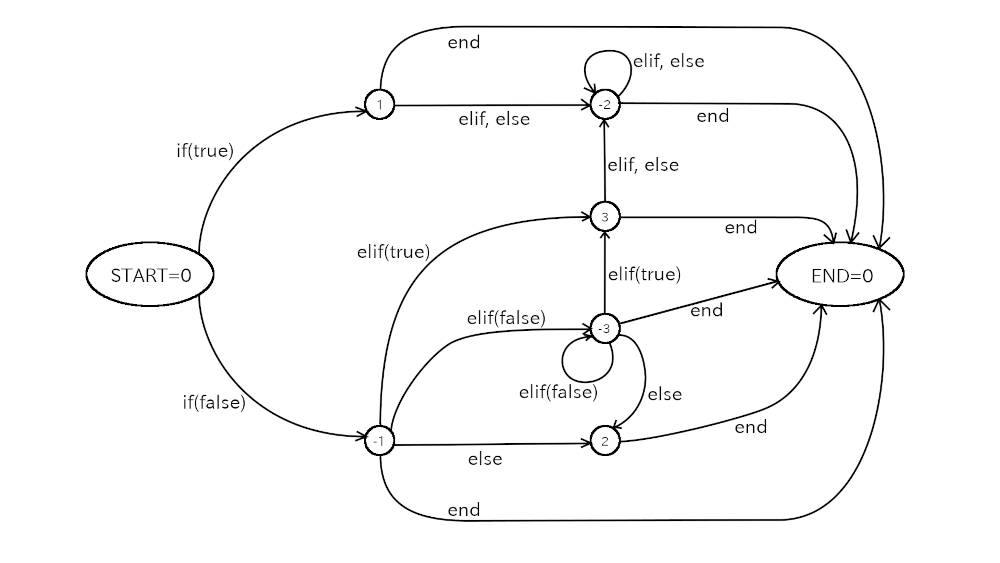
\includegraphics[width=15cm,height=8.4cm]{../image/state_diagram.png}
\caption{diagrama de estado}
\end{figure}

\hypertarget{table}{%
\subsubsection{@@@table}\label{table}}

Este comando @@@ comienza con una línea ``@@@table''. El contenido es
una tabla en formato GFM o pandoc. El comando crea una table fácil de
leer. Por ejemplo, un archivo \texttt{sample.md} posee una tabla de la
siguiente manera:

\begin{verbatim}
Price list

@@@table
|item|price|
|:---:|:---:|
|mouse|$10|
|PC|$500|
@@@
\end{verbatim}

El comando se transforma en lo siguiente:

\begin{verbatim}
Price list

|item |price|
|:---:|:---:|
|mouse| $10 |
| PC  |$500 |
\end{verbatim}

Este comando cambia la apariencia de la tabla. No influye en los
archivos html/latex que son convertidos desde markdown. El comando sólo
soporta el formato arriba mencionado.

El script \texttt{mktbl.rb} soporta este comando. Si ejecutas el script:

\begin{verbatim}
$ ruby mktbl.rb sample.md
\end{verbatim}

Las tablas en `sample.md' serán organizadas El script tambien hace un
respaldo \texttt{sample.md.bak}

La tarea del script parece fácil, pero el programa no es tan simple. El
script \texttt{mktbl.rb} usa la líbreria \texttt{lib/lib\_src2md.rb}

Los comandos @@@ son efectivos en todo el texto. Esto significa que no
puedes detenerlos. Pero algunas veces necesitas mostrar los comandos
como en este documento. Una solución es agregar 4 espacios al inicio de
la línea. Entonces los comandos @@@ no son efectivos por que deben estar
al inicio de la línea.

\hypertarget{conversiones}{%
\subsection{Conversiones}\label{conversiones}}

Los comandos @@@ son usados por el método \texttt{src2md} el cual se
encuentra en el archivo \texttt{lib/lib\_src2md.rb} Este método
convierte los archivos \texttt{.src.md} en archivos \texttt{.md}.
Adicionalmente, otras conversiones son realizadas por el método
\texttt{src2md}.

\begin{itemize}
\tightlist
\item
  Los vínculos relativos se sustituyen de acuerdo al cambio en el
  directorio base.
\item
  La opción de tamaño del link de imagen se elimina cuando el destino es
  GFM o html.
\item
  Los vínculos relativos se eliminan menos los relativos a .src.md
  cuando el destino es GFM o html.
\item
  Los vínculos relativos se eliminan cuando el destino es latex.
\end{itemize}

El orden de las conversiones es:

\begin{enumerate}
\def\labelenumi{\arabic{enumi}.}
\tightlist
\item
  @@@if\#\# Src directory and the top directory
\item
  @@@table
\item
  @@@include
\item
  @@@shell
\item
  otros
\end{enumerate}

Hay un archivo \texttt{src2md.rb} en el directorio principal. Invoca el
método \texttt{src2md}. De la misma forma, el método se ejecuta en la
accion del archivo \texttt{Rakefile}

\hypertarget{estructura-del-directorio}{%
\subsection{Estructura del directorio}\label{estructura-del-directorio}}

Existen siete directorios dentro del tutorial. Son \texttt{gfm},
\texttt{docs}, \texttt{latex}, \texttt{src}, \texttt{image},
\texttt{test} y \texttt{lib}. Tres directorios: \texttt{gfm},
\texttt{docs} y \texttt{latex} son los destinos para GFM, html y latex.
Es posible que estos directorios no existan antes de la conversión.

\begin{itemize}
\tightlist
\item
  src: Este directorio contiene los archivos .src.md y los archivos C
  relacionados.
\item
  image: Este directorio contiene imágenes.
\item
  gfm \texttt{rake} convierte los archivos .src.md a archivos GFM y los
  guarda en este directorio.
\item
  docs: \texttt{rake\ html} convertirá los archivos .src.md a html y los
  guarda en este directorio.
\item
  latex: \texttt{rake\ pdf} convertirá los archivos .src.md a latex y
  los guarda en este directorio y crea un pdf en el directorio.
\item
  lib: contiene las líbrerias de ruby.
\item
  test: contiene los archivos de prueba, estos se realizan escribiendo
  \texttt{rake\ test} en la terminal.
\end{itemize}

\hypertarget{directorios-src-y-superior.}{%
\subsection{Directorios Src y
superior.}\label{directorios-src-y-superior.}}

El directorio Src contiene los archivos .src.md y los archivo fuente C.
El directorio principal, que es gt\_tutotial\_spanish, contiene los
archivos \texttt{Rakefile}, \texttt{src2md.rb} y otros. Cuando el
archivo \texttt{Readme.md} es generado, se ubicará en el directorio
principal. \texttt{Readme.md} tiene título, resumen, tabla de contenido
con enlaces a los archivos GFM.

Src directory contains .src.md files and C-related source files. The top
directory, which is gtk\_tutorial directory, contains \texttt{Rakefile},
\texttt{src2md.rb} and some other files. When \texttt{Readme.md} is
generated, it will be located at the top directory. \texttt{Readme.md}
has title, abstract, table of contents with links to GFM files.

Rakefile describes how to convert .src.md files into GFM, html and/or
pdf files. Rake carries out the conversion according to the
\texttt{Rakefile}.

\hypertarget{the-name-of-files-in-src-directory}{%
\subsection{The name of files in src
directory}\label{the-name-of-files-in-src-directory}}

Files in \texttt{src} directory are an abstract, sections of the
document and other .src.md files. An \texttt{abstract.src.md} contains
the abstract of this tutorial. Each section filename is ``sec'', number
of the section and ``.src.md'' suffix. For example, ``sec1.src.md'',
``sec5.src.md'' or ``sec12.src.md''. They are the files correspond to
the section 1, section 5 and section 12 respectively.

\hypertarget{c-source-file-directory}{%
\subsection{C source file directory}\label{c-source-file-directory}}

Most of .src.md files have \texttt{@@@include} commands and they include
C source files. Such C source files are located in the subdirectories of
\texttt{src} directory.

Those C files have been compiled and tested. When you compile source
files, some auxiliary files and a target file like \texttt{a.out} are
created. Or \texttt{\_build} directory is made when \texttt{meson} and
\texttt{ninja} is used when compiling. Those files are not tracked by
\texttt{git} because they are specified in \texttt{.gitignore}.

The name of the subdirectories should be independent of section names.
It is because of renumbering, which will be explained in the next
subsection.

\hypertarget{renumbering}{%
\subsection{Renumbering}\label{renumbering}}

Sometimes you might want to insert a new section. For example, you want
to insert it between section 4 and section 5. You can make a temporary
section 4.5, that is a rational number between 4 and 5. However, section
numbers are usually integer so section 4.5 must be changed to section 5.
And the numbers of the following sections must be increased by one.

This renumbering is done by the \texttt{renumber} method in the
\texttt{lib/lib\_renumber.rb} file.

\begin{itemize}
\tightlist
\item
  It changes file names.
\item
  If there are references (links) to sections in .src.md files, the
  section numbers will be automatically renumbered.
\end{itemize}

\hypertarget{rakefile}{%
\subsection{Rakefile}\label{rakefile}}

Rakefile is similar to Makefile but controlled by rake, which is a ruby
script. Rakefile in this tutorial has the following tasks.

\begin{itemize}
\tightlist
\item
  md: generate GFM markdown files. This is the default.
\item
  html: generate html files.
\item
  pdf: generate latex files and a pdf file, which is compiled by
  lualatex.
\item
  all: generate md, html and pdf files.
\item
  clean: delete latex intermediate files.
\item
  clobber: delete all the generated files.
\end{itemize}

Rake does renumbering before the tasks above.

\hypertarget{generate-gfm-markdown-files}{%
\subsection{Generate GFM markdown
files}\label{generate-gfm-markdown-files}}

Markdown files (GFM) are generated by rake.

\begin{verbatim}
$ rake
\end{verbatim}

This command generates \texttt{Readme.md} with
\texttt{src/abstract.src.md} and titles of each \texttt{.src.md} file.
At the same time, it converts each .src.md file into a GFM file under
the \texttt{gfm} directory. Navigation lines are added at the top and
bottom of each markdown section file.

You can describe width and height of images in .src.md files. For
example,

\begin{verbatim}
![sample image](../image/sample_image.png){width=10cm height=6cm}
\end{verbatim}

The size between left brace and right brace is used in latex file and it
is not fit to GFM syntax. So the size will be removed in the conversion.

If a .src.md file has relative URL links, they will be changed by
conversion. Because .src.md files are located under the \texttt{src}
directory and GFM files are located under the \texttt{gfm} directory.
That means the base directory of the relative link are different. For
example, \texttt{{[}src/sample.c{]}(sample.c)} is translated to
\texttt{{[}src/sample.c{]}(../src/sample.c)}.

If a link points another .src.md file, then the target filename will be
changed to .md file. For example, \texttt{{[}Section\ 5{]}(sec5.src.md)}
is translated to \texttt{{[}Section\ 5{]}(sec5.md)}.

If you want to clean the directory, that means remove all the generated
markdown files, type \texttt{rake\ clobber}.

\begin{verbatim}
$ rake clobber
\end{verbatim}

Sometimes this is necessary before generating GFM files.

\begin{verbatim}
$ rake clobber
$ rake
\end{verbatim}

For example, if you append a new section and other files are still the
same as before, \texttt{rake\ clobber} is necessary. Because the
navigation of the previous section of the newly added section needs to
be updated. If you don't do \texttt{rake\ clobber}, then it won't be
updated because the the timestamp of .md file in gfm is newer than the
one of .src.md file. In this case, using \texttt{touch} to the previous
section .src.md also works to update the file.

If you see the github repository (ToshioCP/Gtk4-tutorial),
\texttt{Readme.md} is shown below the code. And \texttt{Readme.md}
includes links to each markdown files. The repository not only stores
source files but also shows the whole tutorial.

\hypertarget{generate-html-files}{%
\subsection{Generate html files}\label{generate-html-files}}

Src.md files can be translated to html files. You need pandoc to do
this. Most linux distribution has pandoc package. Refer to your
distribution document to install it.

Type \texttt{rake\ html} to generate html files.

\begin{verbatim}
$ rake html
\end{verbatim}

First, it generates pandoc's markdown files under \texttt{docs}
directory. Then, pandoc converts them to html files. The width and
height of image files are removed. Links to .src.md files will be
converted like this.

\begin{verbatim}
[Section 5](sec5.src.md) => [Section 5](sec5.html)
\end{verbatim}

Image files are copied to \texttt{docs/image} direcotiry and links to
them will be converted like this:

\begin{verbatim}
[sample.png](../image/sample.png) => [sample.png](image/sample.png)
\end{verbatim}

Other relative links will be removed.

\texttt{index.html} is the top html file. If you want to clean html
files, type \texttt{rake\ clobber} or \texttt{cleanhtml}.

\begin{verbatim}
$ rake clobber
\end{verbatim}

Every html file has a header
(\texttt{\textless{}head\textgreater{}\ -\/-\ \textless{}/head\textgreater{}}).
It is created by pandoc with `-s' option. You can customize the output
with your own template file for pandoc. Rake uses
\texttt{lib/lib\_mk\_html\_template.rb} to create its own template. The
template inserts bootstrap CSS and Javascript through \texttt{jsDelivr}.

The \texttt{docs} directory contains all the necessary html files. They
are used in the \href{https://ToshioCP.github.io/Gtk4-tutorial}{github
pages} of this repository.

So if you want to publish this tutorial on your own web site, just
upload the files in the \texttt{docs} directory to your site.

\hypertarget{generate-a-pdf-file}{%
\subsection{Generate a pdf file}\label{generate-a-pdf-file}}

You need pandoc to convert markdown files into latex source files.

Type \texttt{rake\ pdf} to generate latex files and finally make a pdf
file.

\begin{verbatim}
$ rake pdf
\end{verbatim}

First, it generates pandoc's markdown files under \texttt{latex}
directory. Then, pandoc converts them into latex files. Links to files
or directories are removed because latex doesn't support them. However,
links to full URL and image files are kept. Image size is set with the
size between the left brace and right brace.

\begin{verbatim}
![sample image](../image/sample_image.png){width=10cm height=6cm}
\end{verbatim}

You need to specify appropriate width and height. It is almost
\texttt{0.015\ x\ pixels} cm. For example, if the width of an image is
400 pixels, the width in a latex file will be almost 6cm.

A file \texttt{main.tex} is the root file of all the generated latex
files. It has \texttt{\textbackslash{}input} commands, which inserts
each section file, between \texttt{\textbackslash{}begin\{document\}}
and \texttt{\textbackslash{}end\{document\}}. It also has
\texttt{\textbackslash{}input}, which inserts \texttt{helper.tex}, in
the preamble. Two files \texttt{main.tex} and \texttt{helper.tex} are
created by \texttt{lib/lib\_gen\_main\_tex.rb}. It has a sample markdown
code and converts it witn \texttt{pandoc\ -s}. Then, it extracts the
preamble in the generated file and puts it into \texttt{helper.tex}. You
can customize \texttt{helper.tex} by modifying
\texttt{lib/lib\_gen\_main\_tex.rb}.

Finally, lualatex compiles the \texttt{main.tex} into a pdf file.

If you want to clean \texttt{latex} directory, type
\texttt{rake\ clobber} or \texttt{rake\ cleanlatex}

\begin{verbatim}
$ rake clobber
\end{verbatim}

This removes all the latex source files and a pdf file.
